\documentclass{article}
\usepackage[T1]{fontenc}
\usepackage[utf8]{inputenc}
\usepackage{amsmath}
\usepackage{graphicx}
\usepackage{float}
\usepackage{listings}
\usepackage{xcolor}

\title{Explanation}
\author{Pawan Mali }
\date{June 2026}

\begin{document}
\maketitle
\section{Provided Repository structure Explanation}

I analyzed the local folder. It contains two ROS 2 workspaces:

\begin{figure}[H]
    \centering
    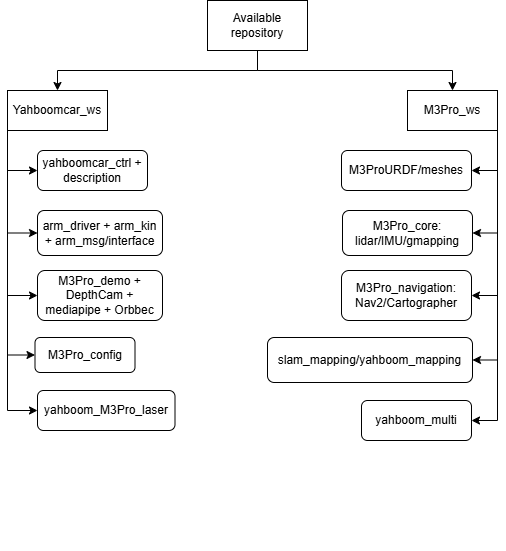
\includegraphics[width=0.9\textwidth]{Img/Repo_Downloaded.png}
    \caption{Overview of the downloaded repository structure}
    \label{fig:repo_structure}
\end{figure}

\subsection{yahboomcar\_ws/src}

\begin{itemize}
    \item \textbf{yahboomcar\_ctrl}: Keyboard and joystick teleoperation. Important files include \texttt{yahboom\_keyboard.py} and \texttt{yahboom\_joy\_M3Pro.py}.
    
    \item \textbf{yahboom\_M3Pro\_description}: Contains the robot URDF, meshes, and RViz model display files.
    
    \item \textbf{M3Pro\_config}: MoveIt2 configuration package containing arm planning settings and fake \texttt{ros2\_control} configuration.
    
    \item \textbf{M3Pro\_demo}: Includes computer vision and manipulation demonstrations such as AprilTag detection, color tracking, KCF tracking, grasping, and line-following.
    
    \item \textbf{yahboom\_M3Pro\_laser}: Lidar-based applications including obstacle avoidance, obstacle warning, and target tracking.
    
    \item \textbf{yahboom\_M3Pro\_DepthCam}: Depth camera examples including distance measurement, depth-color visualization, and edge detection.
    
    \item \textbf{OrbbecSDK\_ROS2}: ROS 2 driver package for Orbbec/Dabai depth cameras.
    
    \item \textbf{arm\_interface, arm\_msgs}: Custom messages and services used for robotic arm communication.
    
    \item \textbf{arm\_kin}: Forward and inverse kinematics services implemented using KDL.
    
    \item \textbf{arm\_driver}: Serial communication driver for the robotic arm using the Rosmaster library.
\end{itemize}

\subsection{M3Pro\_ws/src}

\begin{itemize}
    \item \textbf{M3Pro}: Robot URDF, meshes, and model display launch files.
    
    \item \textbf{M3Pro\_core}: Core robot packages including laser merging, laser filtering, IMU filtering, and GMapping support.
    
    \item \textbf{M3Pro\_navigation}: Navigation stack configuration including Nav2, Cartographer localization, and RViz navigation setups.
    
    \item \textbf{slam\_mapping, yahboom\_mapping}: Packages used for SLAM and map generation/saving.
    
    \item \textbf{ekf\_bringup}: Robot localization package that fuses \texttt{/odom\_raw} and \texttt{/imu/data} using an Extended Kalman Filter (EKF).
    
    \item \textbf{calibration}: Linear and angular calibration utilities based on \texttt{/cmd\_vel} and TF data.
    
    \item \textbf{yahboom\_multi}: Multi-robot navigation and coordination configurations.
    
    \item \textbf{patrol}: Laser-based autonomous patrol behavior implementation.
    
    \item \textbf{largemodel, largemodel\_arm}: AI, voice interaction, and computer vision application examples.
\end{itemize}
\section{Complete Hardware and software based pipeline}
\subsection{Hardware pipeline}

\begin{figure}[H]
    \centering
    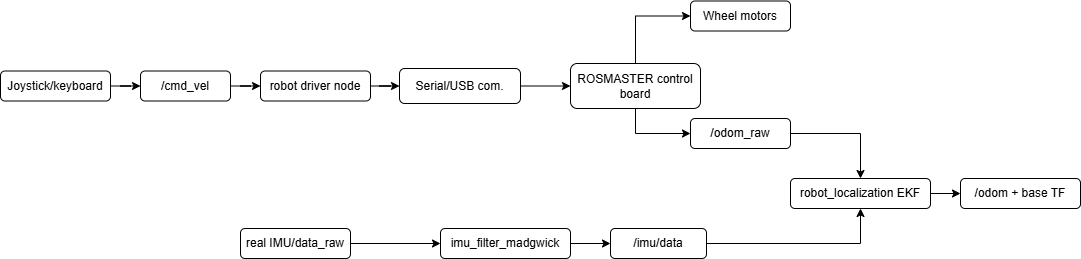
\includegraphics[width=0.9\textwidth]{Img/H_control_pipeline.png}
    \caption{Hardware control pipeline overview}
    \label{fig:H_control_pipeline}
\end{figure}

\paragraph{}

In the hardware-based system, movement commands are generated by a keyboard, joystick, and published on the \texttt{/cmd\_vel} topic. These commands are sent through the robot driver and serial communication interface to the ROSMASTER control board, which controls the motor driver and wheel motors to move the robot. Wheel encoders provide raw odometry data, while the IMU publishes motion data. The IMU data is processed using the Madgwick filter to obtain a cleaner orientation estimate. Finally, the robotlocalization EKF uses the odometry and IMU data to produce accurate robot pose information (\texttt{/odom}) transformation, which are used by RViz2, SLAM, and Nav2 for localization and navigation.


\subsection{Software pipeline}

\begin{figure}[H]
    \centering
    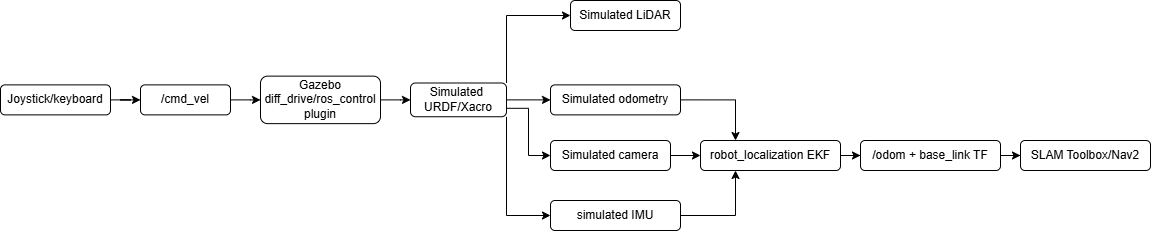
\includegraphics[width=0.9\textwidth]{Img/S_control_pipeline.png}
    \caption{Software control pipeline overview}
    \label{fig:S_control_pipeline}
\end{figure}

\paragraph{}

In the software based system, movement commands are generated by a keyboard and are published on the \texttt{/cmd\_vel} topic. Instead of being sent to a physical robot, these commands are processed by a Gazebo \texttt{diff\_drive} or \texttt{ros2\_control} plugin, which moves the simulated robot model defined by the URDF/Xacro files. As the robot moves within the virtual environment, Gazebo generates simulated sensor data, including odometry, IMU, LiDAR, and camera information. The odometry and IMU data are used by the \texttt{robot\_localization} Extended Kalman Filter (EKF) to produce accurate robot pose estimates and the \texttt{odom} to \texttt{base\_link} transformation. The simulated LiDAR data is used by SLAM Toolbox and Nav2 for mapping, localization, and path planning, while the simulated camera data can be utilized for computer vision tasks such as object detection and obstacle avoidance. This simulation-based architecture enables the development, testing, and validation of robotic algorithms without requiring physical hardware.

\section{Task 1: Simulation based teleoperation}
For this first step, the pipeline contains only:
\begin{itemize}
\item M3Pro base model
\item Gazebo physics
\item robot state publisher
\item Keyboard or joystick teleoperation
\item cmd vel
\item Gazebo movement plugin
\end{itemize}

\subsection{keyboard teleoperation}

\textbf{Previous hardware pipeline:}

\begin{figure}[H]
    \centering
    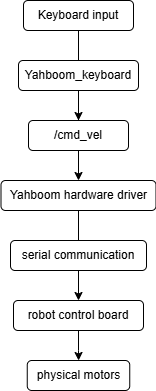
\includegraphics[width=0.25\textwidth]{Img/Keyboard Hardware pipeline.png}
    \caption{Hardware pipeline overview}
    \label{fig:H_control_pipeline}
\end{figure}

The existing \texttt{yahboomcar\_keyboard.py} node can be used without any changes.

\textbf{New software pipeline:}

\begin{figure}[H]
    \centering
    \includegraphics[width=0.25\textwidth]{Img/Keyboard software pipeline.png}
    \caption{Software pipeline overview}
    \label{fig:S_control_pipeline}
\end{figure}

\section{understand the repo structure and debug the errors}
What's actually in this repo
    \begin{itemize}
    \item Two workspaces: {yahboomcar\_ws} (arm driver, robot description/URDF, MoveIt2 config, laser, depth camera) and {M3Pro\_ws} (navigation2, SLAM, calibration, and a big ``largemodel'' AI/voice stack).
    \item The {Docker\_M3Pro-*.sh} scripts pull an image from 192.168.2.51:5000 --- that's a private LAN registry inside Yahboom's factory network, not reachable from your our system at all.
    \item Hardware drivers are hardcoded, e.g. {arm\_driver.py} does {Rosmaster("/dev/ttyUSB0")} using a proprietary \texttt{Rosmaster\_Lib} pip package. Without hardware, this will throw \texttt{SerialException: could not open port /dev/ttyUSB0}.
    \item The only working "no-hardware" launch files are plain URDF viewers (display.launch.py), which just start robot\_state\_publisher + joint\_state\_publisher.

\end{itemize}

\subsection{RViz2 / Robot Description Debugging}
During comiling the repo, I encountered some errors related to missing packages and dependencies. To resolve these issues, I followed these steps:

\begin{figure}[H]
    \centering
    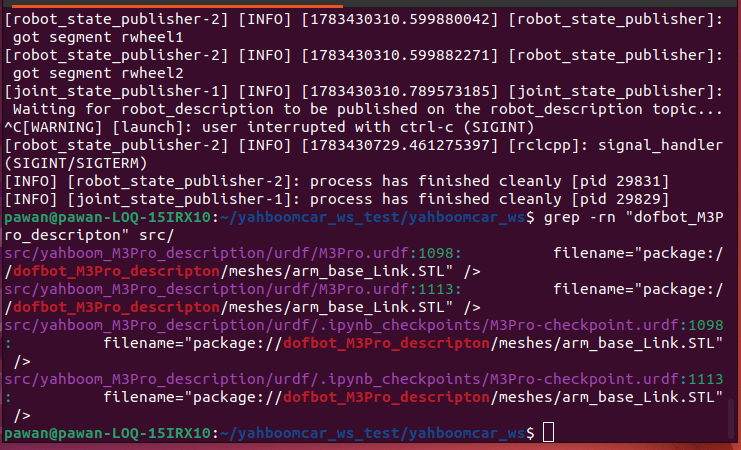
\includegraphics[width=0.8\textwidth]{Img/urdf.png}
    \caption{URDF errors}
    \label{fig:URDF_errors}
\end{figure}
The robot model initially showed an error because the package name in the URDF file was incorrect. The error was found at lines 1098 and 1113. According to the correction, rebuilt the workspace using colcon build, and launched the model again. After the correction, the robot appeared successfully without errors.

\subsection{RViz2 / Controlling the Robot movement}

I tested the Chassis Control Course, especially section 3.3.1 - Controlling the Car’s Speed, without connecting the real robot hardware.


After launching the robot description using display.launch.py. The URDF model loaded correctly in RViz, and the robot was visible without errors. I then checked the active ROS 2 nodes and topics. Only visualization-related nodes such as robot state publisher, joint state publisher, and RViz were running. There was no chassis driver or motor control node.

\begin{figure}[H]
    \centering
    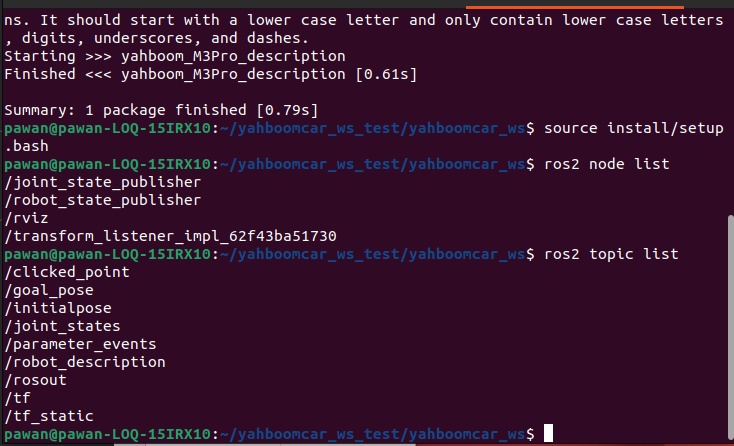
\includegraphics[width=1\textwidth]{Img/topiclist.png}
    \caption{Node and Topic List}
    \label{fig:node and topic list}
\end{figure}


Next, a velocity command was published to the \texttt{/cmd\_vel} topic:

\begin{lstlisting}[language=bash, basicstyle=\ttfamily\small, breaklines=true]
ros2 topic pub /cmd_vel geometry_msgs/msg/Twist \
"{linear: {x: 0.1, y: 0.0, z: 0.0}, angular: {x: 0.0, y: 0.0, z: 0.0}}" --once
\end{lstlisting}

The command continuously showed:

\begin{lstlisting}[basicstyle=\ttfamily\small, breaklines=true]
Waiting for at least 1 matching subscription(s)...
\end{lstlisting}

This happened because no node was subscribed to \texttt{/cmd\_vel}. On the real robot, the chassis driver receives this command, sends motor speed values to the STM32 controller through serial communication, reads encoder data, and publishes odometry. Since the hardware and chassis driver were not available, the velocity command had no receiver.

\begin{figure}[H]
    \centering
    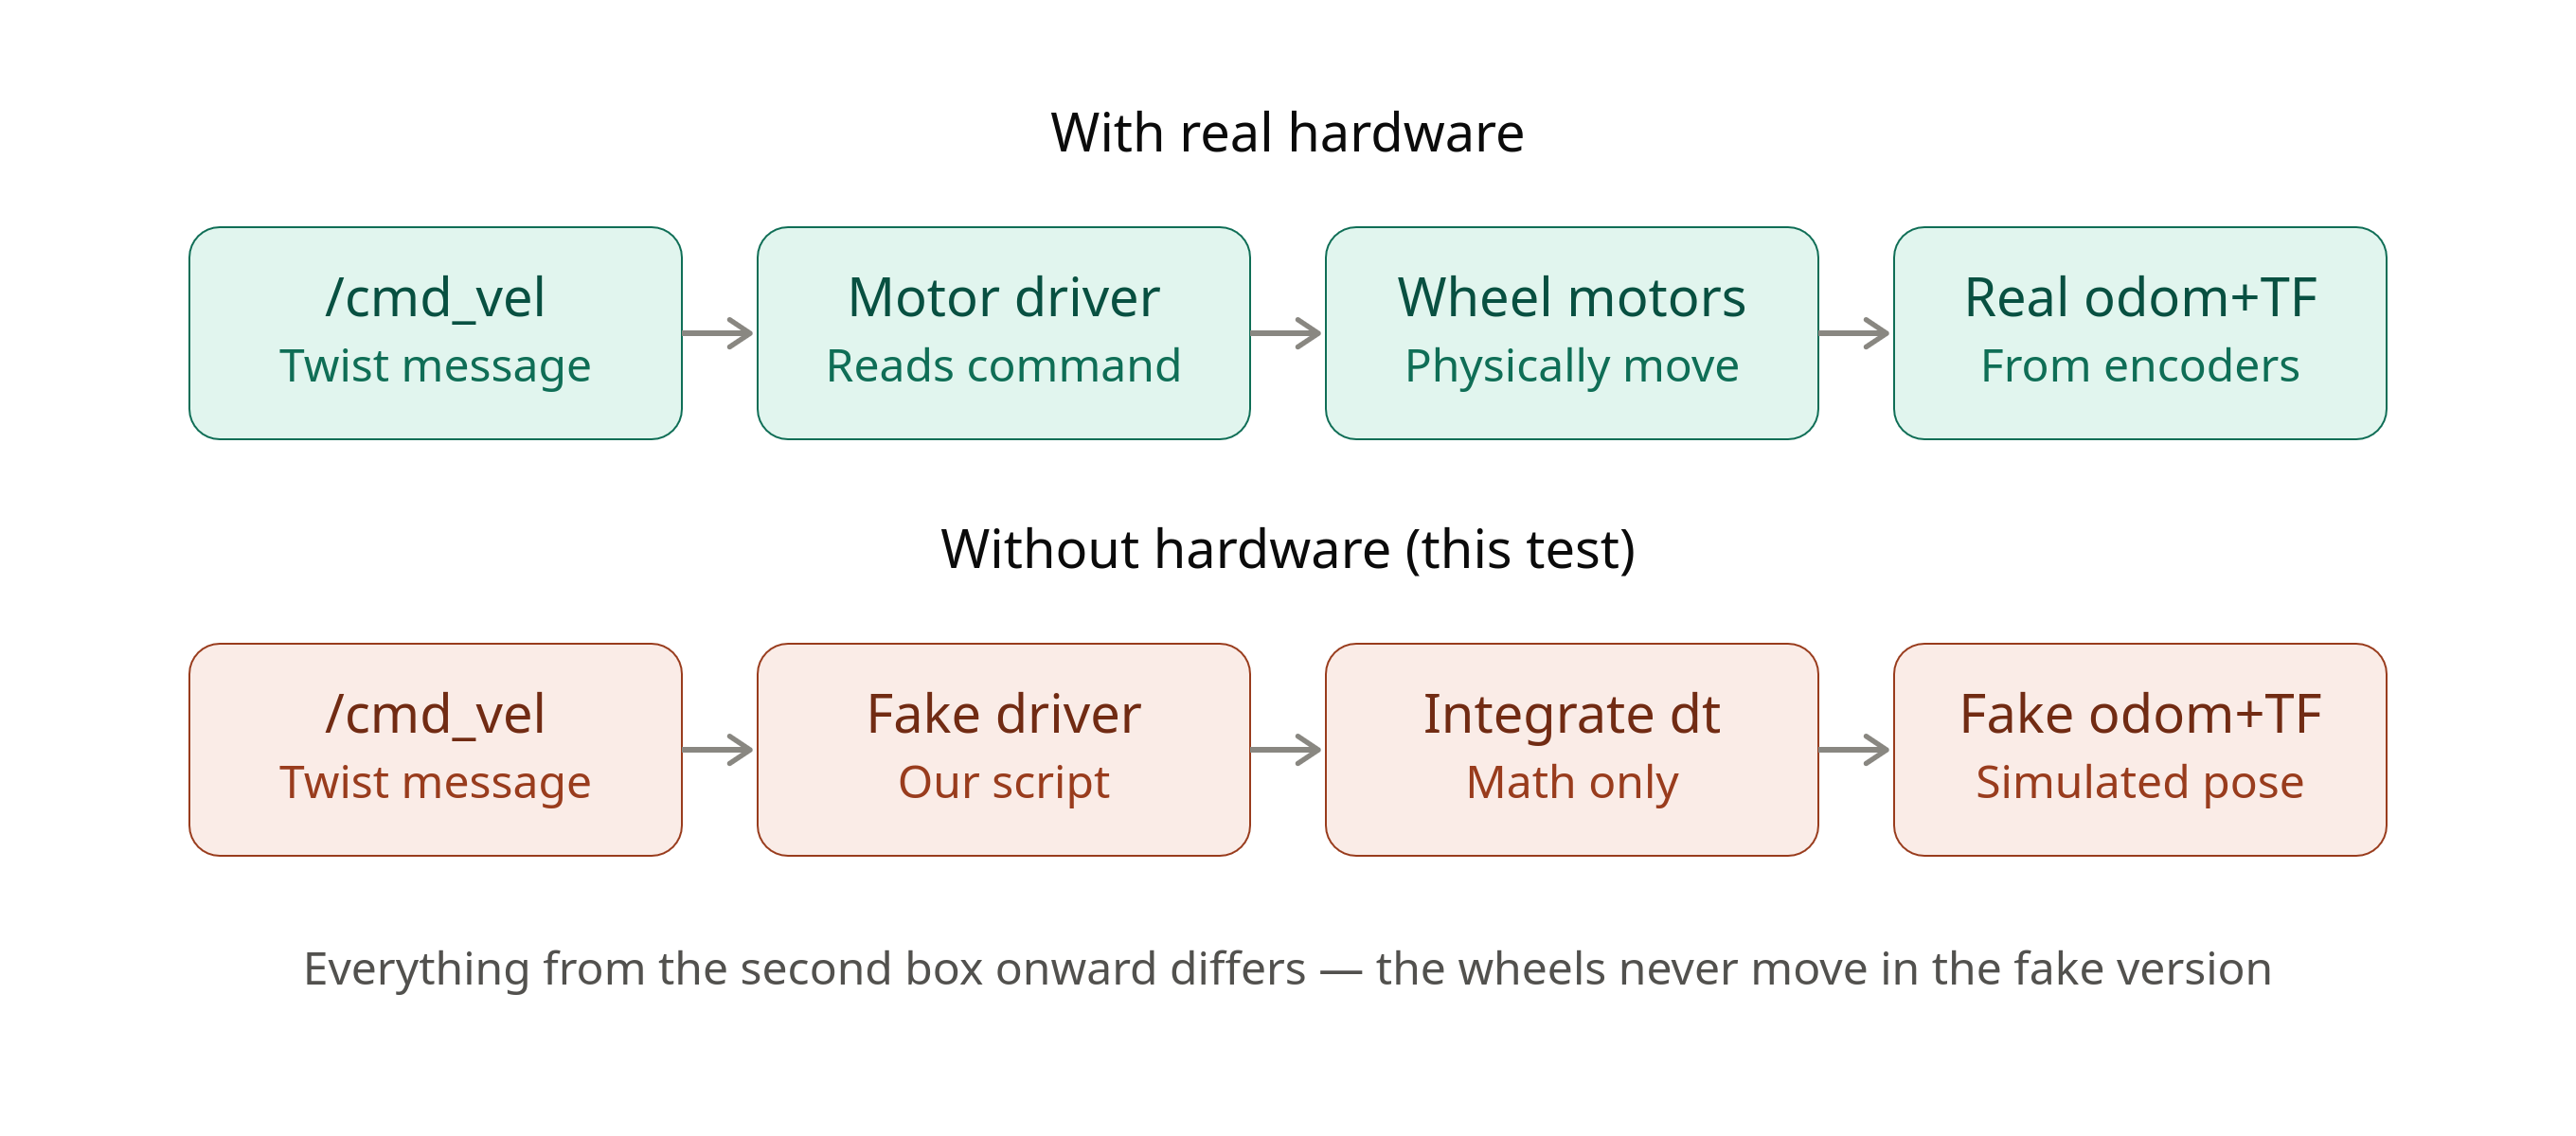
\includegraphics[width=1\textwidth]{Img/real_vs_fake_control_pipeline.png}
    \caption{Real vs. Fake Control Pipeline}
    \label{fig:real_vs_fake_control_pipeline}
\end{figure}

To test the chassis-control command without the real robot hardware, a temporary node called \texttt{fake\_odom\_driver.py} was added. The original command publishes velocity values on \texttt{/cmd\_vel}, but no real motor driver is available to receive them. Therefore, the robot cannot move in RViz using only \texttt{robot\_state\_publisher}.

The fake driver works as a simple software replacement for the hardware driver. It subscribes to \texttt{/cmd\_vel} and reads the commanded forward, sideways, and rotational velocities. These values are stored as:

\begin{lstlisting}[basicstyle=\ttfamily\small, breaklines=true]
linear.x  -> forward/backward movement
linear.y  -> sideways movement for mecanum wheels
angular.z -> rotation
\end{lstlisting}

The node then calculates the robot's new position over time using simple dead-reckoning. It updates the robot's \(x\), \(y\), and heading angle based on the latest velocity command. After calculating the pose, it publishes an odometry message on \texttt{/odom} and broadcasts the TF transformation:

\begin{lstlisting}[basicstyle=\ttfamily\small, breaklines=true]
odom -> base_link
\end{lstlisting}

RViz uses this TF transformation to update the position of the complete robot model. The robot links and joints are still displayed by \texttt{robot\_state\_publisher}, while the fake driver changes the position of the robot base.

\subsection{Set Gazebo Environment / Control the Robot movement}

```latex
\subsection{Base Movement Control in Gazebo Simulation}

\subsubsection{Objective}

The objective of this stage was to make the ROSMASTER M3Pro mobile base movable and controllable in Gazebo Classic using a holonomic control method suitable for its mecanum-wheel configuration. The simulated robot should be capable of forward and backward motion, lateral movement, and rotation around its vertical axis.

\subsubsection{Control Approach}

The mobile base was controlled using the Gazebo Classic \texttt{libgazebo\_ros\_planar\_move.so} plugin. This plugin subscribes to the \texttt{/cmd\_vel} topic and directly applies linear and angular velocities to the robot chassis.

The planar movement plugin supports velocity commands in the longitudinal direction, lateral direction, and yaw rotation. Therefore, the robot can perform holonomic movements such as sideways strafing, which is suitable for a mecanum-wheeled mobile platform.

In this initial simulation approach, the individual wheel-contact kinematics and mecanum roller dynamics are not modelled. Instead, the commanded chassis velocity is applied directly to the robot base. This provides a simple and reliable method for validating keyboard control, navigation commands, odometry, and the overall simulation architecture.

\subsubsection{Files Added}

The following Xacro files were added to the robot description package:

\begin{itemize}
    \item \texttt{urdf/M3Pro.planar\_move.xacro}

    This file defines the \texttt{M3Pro\_gazebo\_planar\_move} macro. The macro contains the Gazebo planar movement plugin configuration, including the command velocity topic, odometry topic, odometry frame, robot base frame, and odometry publishing settings.

    \item \texttt{urdf/M3Pro.wheel\_friction.xacro}

    This file defines the \texttt{M3Pro\_wheel\_friction} macro. It configures the Gazebo friction parameters \texttt{mu1} and \texttt{mu2} for all four wheels. The friction coefficients were reduced to near-zero values because the wheels are not used to physically generate the robot motion when the planar movement plugin is active.
\end{itemize}

\subsubsection{Files Modified}

The following existing files were modified:

\begin{itemize}
    \item \texttt{urdf/M3Pro.urdf.xacro}

    The planar movement and wheel-friction Xacro files were included in the main robot description. Their corresponding macros were then called so that the plugin and friction parameters became part of the robot model loaded into Gazebo.

    \item \texttt{launch/gazebo\_display.launch.py}

    A \texttt{joint\_state\_publisher} node was added to publish joint states for non-driven joints, including the wheel and camera joints. This allowed RViz2 to resolve and display the complete TF tree of the robot.
\end{itemize}

\subsubsection{Implementation and Testing}

After integrating the planar movement plugin, the robot was tested by publishing velocity commands directly to the \texttt{/cmd\_vel} topic. The following types of movement were successfully verified:

\begin{itemize}
    \item Forward and backward movement using the linear velocity component \texttt{linear.x}.
    \item Sideways strafing using the lateral velocity component \texttt{linear.y}.
    \item Clockwise and counter-clockwise rotation using the angular velocity component \texttt{angular.z}.
\end{itemize}

An example command used to test forward movement is shown below:

\begin{verbatim}
ros2 topic pub /cmd_vel geometry_msgs/msg/Twist \
"{linear: {x: 0.3, y: 0.0, z: 0.0},
  angular: {x: 0.0, y: 0.0, z: 0.0}}"
\end{verbatim}

Similarly, lateral movement was tested by assigning a non-zero value to \texttt{linear.y}, while rotational movement was tested by assigning a non-zero value to \texttt{angular.z}.


\subsubsection{Wheel Joint Type and Limit Configuration}

The M3Pro drive wheels must be able to rotate continuously during forward, backward, lateral, and rotational motion. Therefore, the wheel joints should be defined as \texttt{continuous} joints rather than \texttt{revolute} joints.

A \texttt{revolute} joint requires lower and upper angular limits. For example:

\begin{verbatim}
<joint name="wheel_joint" type="revolute">
    <limit lower="-1.0"
           upper="1.0"
           effort="100"
           velocity="100"/>
</joint>
\end{verbatim}

In this configuration, the wheel can rotate only between $-1$ radian and $+1$ radian. This corresponds to a total angular range of:

\[
2~\text{rad} \approx 114.6^\circ
\]

Therefore, the wheel can rotate only approximately one-third of a complete revolution before reaching its position limit. Once the joint reaches either the lower or upper limit, Gazebo prevents any further rotation. Although the velocity limit is set to \texttt{100 rad/s}, this does not remove the angular position restriction.

For this reason, a \texttt{revolute} joint is more suitable for limited-motion joints such as robot arm joints, steering joints, gripper joints, or camera tilt joints.

For the M3Pro drive wheels, the correct configuration is:

\begin{verbatim}
<joint name="wheel_joint" type="continuous">
    <limit effort="10"
           velocity="10"/>
</joint>
\end{verbatim}

A \texttt{continuous} joint can rotate indefinitely in both directions. Therefore, the \texttt{lower} and \texttt{upper} position limits are not required.

The \texttt{effort} parameter defines the maximum torque that may be applied to the joint, while the \texttt{velocity} parameter defines the maximum permitted angular velocity. In this simulation, setting both parameters to non-zero values allowed the wheel joints to move freely when the planar movement plugin commanded the robot chassis.

The previous wheel joint configuration used:

\begin{verbatim}
<limit lower="0"
       upper="0"
       effort="0"
       velocity="0"/>
\end{verbatim}

This configuration did not permit useful wheel motion. The zero velocity limit prevented wheel rotation, while the zero effort limit did not allow torque to be applied to the joint. In addition, the identical lower and upper limits represented a fixed angular position.

After changing the wheel joints to \texttt{continuous} joints and using:

\begin{verbatim}
<limit effort="10"
       velocity="10"/>
\end{verbatim}

the wheels were able to rotate without angular restrictions. This eliminated the abnormal wheel resistance observed during chassis movement and helped resolve the Gazebo tipping behaviour.


\subsubsection{Result}

The M3Pro mobile base is fully functional in the Gazebo Classic simulation. Forward movement, backward movement, lateral strafing, and rotation were successfully tested. The wheel-friction modification eliminated the chassis-tipping problem, while the planar movement plugin provided stable holonomic motion.

The simulated odometry and TF data were also verified using ROS~2 command-line tools and RViz2. Therefore, the base movement stage provides a functional foundation for the subsequent integration of keyboard teleoperation, SLAM, localization, obstacle avoidance, and Nav2-based autonomous navigation.



\subsection{Lidar Scan Merging and SLAM Mapping}

\subsubsection{Objective}

The objective of this task was to combine the data from the two lidar sensors of the M3Pro robot into a single unified laser scan and use the merged scan for Simultaneous Localization and Mapping (SLAM). The final goal was to generate and save an occupancy-grid map of the simulated test environment.

\subsubsection{Background}

The M3Pro robot is equipped with two 360-degree lidar sensors. Their corresponding coordinate frames are defined as \texttt{laser0\_frame} and \texttt{laser1\_frame}. The sensors are mounted at diagonally opposite corners of the robot chassis.

Although each lidar provides a complete rotational scan, parts of its field of view are blocked by the robot body. This creates self-occlusion and causes incomplete measurements around the chassis. By combining both lidar scans, the blind region of one sensor can be covered by the second sensor, producing a more complete representation of the surrounding environment.

\subsubsection{Lidar Scan Merging Approach}

The existing \texttt{ira\_laser\_tools} package was used to merge the two lidar scans. This package was already available in the \texttt{M3Pro\_ws} workspace and provides the \texttt{laserscan\_multi\_merger} node.

The merger node subscribes to the two raw lidar topics:

\begin{itemize}
    \item \texttt{/scan0}
    \item \texttt{/scan1}
\end{itemize}

The measurements from both sensors are transformed into a common reference frame using the available TF transformations. The combined scan is then published on:

\begin{verbatim}
/scan_multi
\end{verbatim}

This merged topic provides a more complete laser scan around the robot and is used as the input for the SLAM system.

\subsubsection{SLAM Approach}

The \texttt{slam\_toolbox} package was used to generate the occupancy-grid map. The existing \texttt{slam\_mapping} package was configured to run \texttt{slam\_toolbox} in online asynchronous mode.

In online asynchronous mode, the SLAM node continuously processes incoming laser scans while the robot moves through the environment. It estimates the robot pose using scan matching and incrementally updates the occupancy-grid map.

The merged lidar topic \texttt{/scan\_multi} was used as the primary sensor input instead of using either lidar individually.

\subsubsection{Configuration Changes}

The following configuration files were reviewed and modified.

\paragraph{\texttt{ira\_laser\_tools/config/laserscan\_merge.yaml}}

The input scan topic names were verified to match the lidar topics published by the Gazebo sensor plugins:

\begin{verbatim}
scan0: /scan0
scan1: /scan1
\end{verbatim}

The merged laser scan was configured to be published on:

\begin{verbatim}
/scan_multi
\end{verbatim}

\paragraph{\texttt{slam\_mapping/config/mapper\_params\_online\_async.yaml}}

The following parameters were updated:

\begin{itemize}
    \item The \texttt{base\_frame} parameter was changed from
    \texttt{base\_footprint} to \texttt{base\_link}, because the current robot
    URDF does not contain a \texttt{base\_footprint} frame.

    \item The \texttt{scan\_topic} parameter was changed from
    \texttt{/scan} to \texttt{/scan\_multi}, allowing
    \texttt{slam\_toolbox} to use the merged lidar data.

    \item The \texttt{max\_laser\_range} parameter was increased from
    \texttt{6.0} metres to \texttt{8.0} metres to match the effective range
    of the simulated lidar sensors and avoid unnecessarily clipping valid
    measurements.
\end{itemize}

The relevant configuration is represented as follows:

\begin{verbatim}
base_frame: base_link
scan_topic: /scan_multi
max_laser_range: 8.0
\end{verbatim}

\subsubsection{Implementation and Testing Process}

The complete lidar merging and mapping pipeline was tested step by step.

\begin{enumerate}
    \item Both raw lidar topics were first verified individually:

\begin{verbatim}
ros2 topic echo /scan0
ros2 topic echo /scan1
\end{verbatim}

    This confirmed that both Gazebo lidar plugins were publishing valid
    \texttt{sensor\_msgs/msg/LaserScan} messages.

    \item The \texttt{ira\_laser\_tools} workspace was built, and the
    \texttt{laserscan\_multi\_merger} node was launched.

    \item The merged topic was verified using:

\begin{verbatim}
ros2 topic echo /scan_multi
\end{verbatim}

    The topic publishing frequency was also checked using:

\begin{verbatim}
ros2 topic hz /scan_multi
\end{verbatim}

    \item The raw and merged scans were visualized in RViz2. The merged scan
    successfully covered regions that were blocked in the individual lidar
    scans, reducing the blind areas caused by the robot chassis.

    \item The \texttt{slam\_mapping} package was built and the following
    launch file was used:

\begin{verbatim}
ros2 launch slam_mapping online_async_launch.py
\end{verbatim}

    This launch file starts the main SLAM node without the additional IMU,
    EKF, and laser-filter processing chain used in the real-hardware launch
    configuration.

    \item RViz2 was opened using the existing visualization launch file:

\begin{verbatim}
ros2 launch slam_mapping slam_view.launch.py
\end{verbatim}

    The LaserScan display topic in RViz2 was changed to
    \texttt{/scan\_multi}.

    \item The robot was manually driven through the simulated maze using the
    existing teleoperation node, which publishes velocity commands on the
    \texttt{/cmd\_vel} topic.

    \item As the robot moved, \texttt{slam\_toolbox} processed the merged
    laser scans and progressively constructed the occupancy-grid map.
\end{enumerate}

\subsubsection{TF Verification}

The TF hierarchy was checked to ensure that the mapping system received the correct robot pose information. The expected transformation chain was:

\[
\texttt{map}
\rightarrow
\texttt{odom}
\rightarrow
\texttt{base\_link}
\]

The \texttt{odom} to \texttt{base\_link} transformation was published by the Gazebo planar movement plugin and represented the local motion of the simulated robot.

The \texttt{map} to \texttt{odom} transformation was published by \texttt{slam\_toolbox}. This transformation corrected accumulated odometry errors based on lidar scan matching and aligned the robot trajectory with the generated map.

The complete TF tree was verified using RViz2 and ROS~2 TF tools.

\subsubsection{Map Generation and Saving}

After the robot had explored the required area and the maze geometry was fully reconstructed, the generated occupancy-grid map was saved using the existing map-saving launch file:

\begin{verbatim}
ros2 launch slam_mapping save_map.launch.py
\end{verbatim}

The map-saving process used \texttt{nav2\_map\_server} and generated the following files:

\begin{itemize}
    \item \texttt{yahboom\_map.yaml}
    \item \texttt{yahboom\_map.pgm}
\end{itemize}

The \texttt{PGM} file contains the occupancy-grid image, while the \texttt{YAML} file contains the associated map metadata, including resolution, origin, occupancy threshold, free-space threshold, and map image location.

\subsubsection{Result}

The complete dual-lidar SLAM pipeline was successfully implemented and tested in Gazebo Classic. Both raw lidar scans were merged into the unified \texttt{/scan\_multi} topic, and the resulting scan provided improved environmental coverage around the robot.

The merged lidar data was successfully used by \texttt{slam\_toolbox} to generate a live occupancy-grid map. The reconstructed maze geometry closely matched the ground-truth Gazebo world, confirming that the lidar transformations, scan merging, odometry, TF hierarchy, and SLAM configuration were functioning correctly.

The final map was saved successfully as \texttt{yahboom\_map.yaml} and \texttt{yahboom\_map.pgm}.

\subsubsection{Next Step}

The saved occupancy-grid map will be used in the next stage of the project for Nav2-based localization, global path planning, local path planning, and autonomous navigation. The initial launch and configuration structure for this stage is already available in the \texttt{M3Pro\_navigation} package.


\subsection{Wheel-Friction Tuning Refinement}
\label{sec:wheel_friction_refinement}

\subsubsection{Objective}

Following the initial base-movement implementation described in Section~4.4, the wheel-ground friction coefficients were revisited and refined. In the first implementation, the friction coefficients \texttt{mu1} and \texttt{mu2} were reduced to values close to zero in order to eliminate the chassis-tipping behaviour observed during motion.

Although this modification successfully removed the tipping problem, further testing showed that the selected friction values were too low for stable and realistic planar movement. Therefore, an empirical tuning step was carried out to identify a more suitable intermediate value.

\subsubsection{Problem with the Initial Near-Zero Friction}

The near-zero wheel-ground friction coefficients successfully prevented the front or rear of the chassis from lifting during commanded movement. However, they introduced a secondary problem.

Because the contact between the wheels and the Gazebo ground plane offered almost no frictional resistance, the wheels tended to slide or skate laterally across the surface. As a result, the robot did not always track the commanded \texttt{/cmd\_vel} velocity cleanly, especially during lateral movement and combined translational and rotational commands.

This behaviour occurred because the planar-movement plugin directly applies the requested planar velocity to the chassis, while the wheel-ground contact still contributes to the physical response of the robot model. If the wheel friction is too low, the contact points provide insufficient resistance to undesired lateral drift.

\subsubsection{Friction Refinement}

The friction coefficients defined in \texttt{M3Pro.wheel\_friction.xacro} were increased from their initial near-zero values to:

\begin{verbatim}
mu1 = 0.51
mu2 = 0.51
\end{verbatim}

The same values were applied to all four wheel links:

\begin{itemize}
    \item \texttt{lwheel1}
    \item \texttt{lwheel2}
    \item \texttt{rwheel1}
    \item \texttt{rwheel2}
\end{itemize}

An example Gazebo wheel-friction configuration is shown below:

\begin{verbatim}
<gazebo reference="lwheel1">
    <mu1>0.51</mu1>
    <mu2>0.51</mu2>
</gazebo>
\end{verbatim}

The selected value was determined experimentally. It provided enough wheel-ground resistance to prevent excessive lateral sliding while remaining sufficiently low to avoid reintroducing the chassis-pitching problem described in Section~4.4.

\subsubsection{File Modified}

The following file was modified:

\begin{itemize}
    \item \texttt{urdf/M3Pro.wheel\_friction.xacro}

    The \texttt{mu1} and \texttt{mu2} coefficients for all four wheel links were changed from their initial near-zero values to \texttt{0.51}.
\end{itemize}

\subsubsection{Result}

After the friction coefficients were updated, the robot base followed the commanded \texttt{/cmd\_vel} velocities more consistently. Forward, backward, lateral, and rotational movement could be executed without the previous skating behaviour and without reintroducing the chassis-tipping problem.

The value \texttt{0.51} is treated as an empirically tuned simulation parameter. It is specific to the current URDF model, including its mass distribution, collision geometry, wheel dimensions, inertial properties, and Gazebo physics configuration. It should therefore not be interpreted as a universal friction value for all mecanum-wheeled robot models.


\subsection{Depth-Camera Integration in Gazebo Simulation}
\label{sec:depth_camera_integration}

\subsubsection{Objective}

The objective of this stage was to integrate a simulated RGB-D depth camera into the M3Pro digital twin. The simulated camera was configured to produce RGB images, depth images, camera calibration data, and point-cloud data using a topic structure similar to that of the physical depth-camera driver.

This enables computer-vision and perception nodes to be developed and tested in simulation before the physical camera hardware is available.

\subsubsection{Background}

The imported M3Pro URDF already contained a link named \texttt{Camera}. This link included the camera mesh and inertial properties and was fixed relative to \texttt{base\_link}. However, the link had no Gazebo sensor functionality attached to it.

Consequently, the camera appeared visually as part of the robot model but did not publish any image, depth, or point-cloud data. A Gazebo sensor definition and ROS plugin were therefore required to convert the existing camera link into a functional simulated RGB-D sensor.

\subsubsection{Implementation Approach}

A Gazebo depth-camera sensor was attached to the existing \texttt{Camera} link using the following plugin:

\begin{verbatim}
libgazebo_ros_camera.so
\end{verbatim}

In addition, a dedicated optical frame named:

\begin{verbatim}
camera_color_optical_frame
\end{verbatim}

was created and connected to the existing \texttt{Camera} link by a fixed joint.

The optical-frame orientation correction was defined as:

\begin{verbatim}
rpy="-1.5708 0 -1.5708"
\end{verbatim}

This correction was necessary because the native coordinate frame inherited from the imported URDF did not follow the standard ROS camera optical-frame convention.

According to the ROS optical-frame convention:

\begin{itemize}
    \item the positive $z$-axis points forward,
    \item the positive $x$-axis points to the right,
    \item the positive $y$-axis points downward.
\end{itemize}

The fixed-joint rotation aligns the simulated camera data with this convention so that downstream ROS~2 image-processing and point-cloud nodes interpret the measurements correctly.

\subsubsection{Sensor Configuration}

The simulated RGB-D camera was configured using the following main parameters:

\begin{itemize}
    \item Image resolution: $640 \times 480$ pixels
    \item Horizontal field of view: approximately $60^\circ$
    \item Minimum clipping distance: $0.1$~m
    \item Maximum clipping distance: $10.0$~m
    \item Update rate: $15$~Hz
\end{itemize}

The camera plugin was configured to publish topics corresponding to the expected hardware-driver layout, including:

\begin{itemize}
    \item \texttt{/camera/color/image\_raw}
    \item \texttt{/camera/color/camera\_info}
    \item \texttt{/camera/depth/image\_raw}
    \item \texttt{/camera/depth/camera\_info}
    \item \texttt{/camera/depth/points}
\end{itemize}

The purpose of reproducing the hardware-side topic structure was to make the simulation and hardware interfaces as consistent as possible. In principle, a downstream computer-vision node should then be able to consume either simulated or real camera data without substantial code changes.

\subsubsection{File Added}

The following file was added:

\begin{itemize}
    \item \texttt{urdf/M3Pro.camera\_links.xacro}

    This file defines the \texttt{M3Pro\_camera\_links} macro. The macro contains the fixed optical-frame joint, optical-frame link, Gazebo RGB-D sensor definition, and ROS camera plugin configuration.
\end{itemize}

\subsubsection{File Modified}

The following file was modified:

\begin{itemize}
    \item \texttt{urdf/M3Pro.urdf.xacro}

    The new camera Xacro file was included in the main robot description, and the \texttt{M3Pro\_camera\_links} macro was instantiated.
\end{itemize}

\subsubsection{Known Namespace Issue}

During testing, the image and depth topics were found under a duplicated camera namespace:

\begin{verbatim}
/camera/camera/...
\end{verbatim}

instead of the intended structure:

\begin{verbatim}
/camera/...
\end{verbatim}

This duplication is caused by the interaction between the explicit \texttt{<namespace>} setting in the plugin configuration and the camera plugin's own internal topic namespace behaviour.

As a result, the current simulated topic names do not exactly match those expected by the existing hardware-side subscriber node:

\begin{verbatim}
pub_rgb_image.py
\end{verbatim}

The subscriber currently expects the non-duplicated camera topic. Therefore, it cannot yet consume the simulated RGB image directly without either correcting the Gazebo plugin namespace or remapping the topic.

\subsubsection{Result}

The camera model is correctly attached to the robot and rendered in Gazebo. The sensor plugin successfully publishes RGB images, depth images, camera information, and point-cloud data at the configured update rate.

The optical frame is also present in the TF tree with the required orientation correction. However, the duplicated namespace remains an open integration issue and must be corrected before the simulated camera feed can be used transparently by the existing computer-vision nodes.


\subsection{Project Documentation Using Markdown Files}
\label{sec:project_documentation}

\subsubsection{Objective}

The objective of this task was to create clear and modular repository documentation for the implemented simulation features. The documentation was intended to make the project understandable to supervisors, collaborators, and future users who access the GitHub repository independently of the written thesis report.

\subsubsection{Documentation Approach}

Rather than maintaining one large combined document, a separate Markdown file was created for each major implemented feature. An additional index file was created to connect the individual documents and provide the overall setup and execution instructions.

This documentation structure follows the same modular design principle used for the Xacro files, where each file has one main responsibility. It makes the repository easier to navigate, maintain, and extend.

\subsubsection{Files Added}

The following documentation files were added:

\begin{itemize}
    \item \texttt{docs/README.md}

    This file serves as the documentation index. It contains links to the individual feature documents, dependency and setup instructions, the complete build-and-run command sequence, and an explanation of the two-workspace repository structure.

    \item \texttt{docs/01-gazebo-environment-setup.md}

    This document explains the Gazebo world file, robot spawning sequence, simulation launch architecture, and environment setup.

    \item \texttt{docs/02-robot-base-movement.md}

    This document describes the planar-movement-based mecanum simulation, the earlier \texttt{ros2\_control} approach that was evaluated but not selected for the initial implementation, and the debugging process related to wheel friction and chassis tipping.

    \item \texttt{docs/03-lidar-integration.md}

    This document covers the simulated lidar sensors, raw scan topics, dual-lidar scan merging, filtering, TF requirements, and SLAM topic configuration.

    \item \texttt{docs/04-depth-camera-integration.md}

    This document describes the simulated RGB-D camera, the optical-frame correction, published topics, plugin configuration, and the known duplicated-namespace issue.
\end{itemize}

\subsubsection{Result}

The repository now contains standalone documentation for each major implemented feature. Each document explains what was changed, why the change was required, how the corresponding pipeline works, and how it can be launched and tested.

This documentation improves the reproducibility and maintainability of the project and allows the codebase to be understood independently of the thesis report.


\subsection{Consolidated Launch and Cleanup Script}
\label{sec:run_lidar_pipeline}

\subsubsection{Objective}

Testing the complete lidar-merging and SLAM pipeline previously required launching several ROS~2 processes manually in separate terminals. These included Gazebo, the dual-lidar scan merger, \texttt{slam\_toolbox}, and RViz2.

A shell script named:

\begin{verbatim}
run_lidar_pipeline.sh
\end{verbatim}

was created to automate both the launch sequence and the shutdown procedure.

\subsubsection{Problem Being Solved}

The complete pipeline required four processes to be launched in the correct order:

\begin{enumerate}
    \item Gazebo Classic with the robot and maze environment
    \item Dual-lidar scan-merging node
    \item \texttt{slam\_toolbox}
    \item RViz2
\end{enumerate}

Starting these components manually across several terminals was repetitive and prone to timing-related errors. Some nodes could start before the topics or TF frames they depended on were available.

A further problem was caused by Gazebo Classic's process behaviour. The \texttt{gzserver} and \texttt{gzclient} processes may continue running after a normal \texttt{Ctrl+C} or after the parent ROS~2 launch process is terminated.

These remaining processes can interfere with the next simulation run and may cause problems such as:

\begin{itemize}
    \item Gazebo transport ports already being in use,
    \item duplicate node names,
    \item old topics remaining active,
    \item multiple Gazebo server instances,
    \item conflicts between old and new simulation sessions.
\end{itemize}

Manually finding and terminating these stale processes before each test run was time-consuming and error-prone.

\subsubsection{File Added}

The following script was added:

\begin{itemize}
    \item \texttt{run\_lidar\_pipeline.sh}

    This script launches the complete Gazebo, dual-lidar merging, SLAM, and RViz2 pipeline in the required sequence.
\end{itemize}

\subsubsection{Launch Sequence}

The script starts each pipeline component with a fixed delay before launching the next component. These delays allow the required nodes, topics, and TF frames to become available.

The automated sequence is:

\begin{enumerate}
    \item Start Gazebo Classic with the robot and maze world.
    \item Wait for the Gazebo simulation and lidar topics to initialize.
    \item Start the dual-lidar scan merger.
    \item Wait for the merged scan topic to become available.
    \item Start \texttt{slam\_toolbox}.
    \item Start RViz2 with the SLAM visualization configuration.
\end{enumerate}

The complete pipeline can be started using:

\begin{verbatim}
./run_lidar_pipeline.sh
\end{verbatim}

\subsubsection{Process-Group Management}

Each launched process is started using:

\begin{verbatim}
setsid
\end{verbatim}

The \texttt{setsid} command creates a new session and process group for each launched component. This allows the script to terminate the entire process group instead of terminating only the immediate parent process.

This is important because a ROS~2 launch process may start several child processes. Killing only the parent process may leave its children running.

The process-group identifiers are stored by the script and later used during shutdown.

\subsubsection{Signal Trapping and Cleanup}

The script defines a \texttt{cleanup()} function and registers it using a shell \texttt{trap} for the following signals:

\begin{itemize}
    \item \texttt{SIGINT}
    \item \texttt{SIGTERM}
    \item \texttt{SIGHUP}
    \item \texttt{EXIT}
\end{itemize}

This ensures that the cleanup procedure is executed when the user presses \texttt{Ctrl+C}, the terminal session closes, the script receives a termination signal, or the script exits normally.

The cleanup function first terminates the tracked process groups. It then explicitly terminates known pipeline processes as an additional safety mechanism, including:

\begin{itemize}
    \item \texttt{gzserver}
    \item \texttt{gzclient}
    \item the lidar-merger node
    \item \texttt{slam\_toolbox}
    \item RViz2
\end{itemize}

The direct process termination is required because Gazebo's detached child processes do not always respond reliably to the process-group signal.

\subsubsection{Pre-Flight Cleanup}

The same process-termination sequence is also executed before starting a new pipeline session.

This pre-flight cleanup removes stale processes left behind by an earlier run, for example when the terminal window was closed without allowing the script to perform its normal shutdown procedure.

This ensures that every test begins from a clean simulation state.

\subsubsection{Error-Tolerant Cleanup Commands}

The cleanup commands are followed by:

\begin{verbatim}
|| true
\end{verbatim}

This prevents the script from stopping when a cleanup command does not find a matching process.

For example, attempting to terminate \texttt{gzserver} when no Gazebo server is running is a normal situation and should not be treated as a script failure.

\subsubsection{Result}

The complete lidar-merging and SLAM pipeline can now be launched using a single command. Gazebo, the scan merger, \texttt{slam\_toolbox}, and RViz2 are started automatically in the correct sequence.

Pressing \texttt{Ctrl+C} triggers the cleanup procedure and reliably terminates the tracked process groups as well as Gazebo's detached child processes.

This automation removed a recurring source of stale-process conflicts and made repeated simulation testing faster, more reliable, and easier to reproduce.



\end{document}

